\documentclass[english]{article}\usepackage[]{graphicx}\usepackage[]{color}
%% maxwidth is the original width if it is less than linewidth
%% otherwise use linewidth (to make sure the graphics do not exceed the margin)
\makeatletter
\def\maxwidth{ %
  \ifdim\Gin@nat@width>\linewidth
    \linewidth
  \else
    \Gin@nat@width
  \fi
}
\makeatother

\definecolor{fgcolor}{rgb}{0.345, 0.345, 0.345}
\newcommand{\hlnum}[1]{\textcolor[rgb]{0.686,0.059,0.569}{#1}}%
\newcommand{\hlstr}[1]{\textcolor[rgb]{0.192,0.494,0.8}{#1}}%
\newcommand{\hlcom}[1]{\textcolor[rgb]{0.678,0.584,0.686}{\textit{#1}}}%
\newcommand{\hlopt}[1]{\textcolor[rgb]{0,0,0}{#1}}%
\newcommand{\hlstd}[1]{\textcolor[rgb]{0.345,0.345,0.345}{#1}}%
\newcommand{\hlkwa}[1]{\textcolor[rgb]{0.161,0.373,0.58}{\textbf{#1}}}%
\newcommand{\hlkwb}[1]{\textcolor[rgb]{0.69,0.353,0.396}{#1}}%
\newcommand{\hlkwc}[1]{\textcolor[rgb]{0.333,0.667,0.333}{#1}}%
\newcommand{\hlkwd}[1]{\textcolor[rgb]{0.737,0.353,0.396}{\textbf{#1}}}%
\let\hlipl\hlkwb

\usepackage{framed}
\makeatletter
\newenvironment{kframe}{%
 \def\at@end@of@kframe{}%
 \ifinner\ifhmode%
  \def\at@end@of@kframe{\end{minipage}}%
  \begin{minipage}{\columnwidth}%
 \fi\fi%
 \def\FrameCommand##1{\hskip\@totalleftmargin \hskip-\fboxsep
 \colorbox{shadecolor}{##1}\hskip-\fboxsep
     % There is no \\@totalrightmargin, so:
     \hskip-\linewidth \hskip-\@totalleftmargin \hskip\columnwidth}%
 \MakeFramed {\advance\hsize-\width
   \@totalleftmargin\z@ \linewidth\hsize
   \@setminipage}}%
 {\par\unskip\endMakeFramed%
 \at@end@of@kframe}
\makeatother

\definecolor{shadecolor}{rgb}{.97, .97, .97}
\definecolor{messagecolor}{rgb}{0, 0, 0}
\definecolor{warningcolor}{rgb}{1, 0, 1}
\definecolor{errorcolor}{rgb}{1, 0, 0}
\newenvironment{knitrout}{}{} % an empty environment to be redefined in TeX

\usepackage{alltt}
\usepackage[margin=0.7in]{geometry}
\usepackage[titles]{tocloft}
\renewcommand{\cftdot}{}
\usepackage{fontspec}
\setmainfont[Mapping=tex-text]{Gill Sans MT}
\usepackage{fancyhdr}
\pagestyle{fancy}
\usepackage{fancybox}
\usepackage{float}
\usepackage{subfig}
\usepackage{subfloat}
\usepackage{graphicx}
\usepackage{amsmath}
%\RequirePackage{color}
%\RequirePackage[svgnames]{xcolor}
%\definecolor{spYellow}{HTML}{ADAD00}
\RequirePackage{listings}
\usepackage{longtable}
\usepackage{array,booktabs}
\usepackage{bm}
\usepackage{outlines}
\usepackage{newfloat}
\usepackage{caption}
\DeclareFloatingEnvironment[fileext=frm,placement={!ht},name=Code]{Code}
\captionsetup[Code]{labelfont=bf}
\usepackage[font=small,format=plain,labelsep=period,
labelfont=bf, justification=centerlast]{caption}
% With this, we do \begin{Code} \caption{Code name} \ref{whatever} \begin{SAS or R} \end{SAS or R} \end{Code} to get the code in the TOC!

% Now we make an environment for coding in SAS
% We are going to build a new listings (code) environment!

\usepackage{babel}
\usepackage{pdfpages}
\usepackage{tikz}
\usepackage[buttonsize=1em]{animate}
\usepackage[colorlinks=true,citecolor=blue,linkcolor=blue,filecolor=magenta,urlcolor=cyan]{hyperref}
\IfFileExists{upquote.sty}{\usepackage{upquote}}{}
\begin{document}
	% !Rnw weave = knitr
	% !TeX program = xelatex
	%First we define our chunk settings
	

\fancyhead[C]{David Josephs}
\begin{titlepage}
	\pagecolor{white}
	\begin{center}
		\vspace*{1cm}
		
		\Huge
		% For font size, you have
		% {\tiny }
		% {\scriptsize }
		% {\footnotesize }
		% {\small }
		% {\normalsize }
		% {\large }
		% {\Large }
		% {\LARGE }
		% {\huge }
		%{\Huge }
		% Which all multiply your default font size by some constant
		\textbf{Homework 11}
		
		\vspace{0.5cm}
		\LARGE
Regression Diagnostics and Model Refinement

		
		\vspace{1.5cm}
		
		\textbf{David Josephs}
		
		\vspace{1.5cm}
		% I put the SMU Logo here
		
\includegraphics[width=0.4\textwidth]{Logo}
		
		
		\vspace{0.8cm}
		
		
		
		\Large
		Southern Methodist University\\
		%% \\ is a line break, vspace is vertical space. Useful to know
		Masters in Data Science\\
		\today
		
	\end{center}
\end{titlepage}
% TOC
\tableofcontents
\setcounter{tocdepth}{2}
\setcounter{secnumdepth}{3}
\listofCode
\listoffigures
\pagebreak
\section{Testing Kleiber's Law}

\subsection{Examining the Raw Data}
First, we will plot the raw data as a scatterplot, to see if $MASS^{\frac{3}{4}}$ is a reasonable for the data. To do this, we will use the following SAS code:
	\begin{Code}[H]
		\caption{Plotting the Raw Data in SAS}
\begin{center}
\begin{knitrout}
\definecolor{shadecolor}{rgb}{0.969, 0.969, 0.969}\color{fgcolor}\begin{kframe}
\begin{alltt}
data powermetabolism;
set metabolism;
powerMass=Mass**(3/4);
Metab=Metab;
run;
proc sgplot data=powermetabolism noautolegend;
title "Kleiber's Law";
scatter x=powerMass y=Metab;
xaxis label="Body Mass^(3/4) in kg" grid;
yaxis label="Metabolic Rate in kg per Day" grid;
run;
\end{alltt}
\end{kframe}
\end{knitrout}
\end{center}
\end{Code}
Lets see what that graph looks like:
\begin{figure}[H]
	\caption{Scatter Plot of The Raw Data}
	\label{fig:sasterplot1}
	\begin{center}
\includegraphics{SASout/sascatter.png}
\par\end{center}
\end{figure}

From this graph, it does appear to be linear but it needs to be transformed a bit. a non transformed model will not fit, but in general it should fit.
\subsection{Assumption Testing}
To test the assumptions of the regression of the \emph{raw} data, the following SAS code was used:
\begin{Code}[H]
	\caption{Regression Diagnostics with SAS}
	\label{cd:SASregdiagraw}
\begin{knitrout}
\definecolor{shadecolor}{rgb}{0.969, 0.969, 0.969}\color{fgcolor}\begin{kframe}
\begin{alltt}
proc glm data=powermetabolism plots=all alpha=.05;
model Metab=powerMass / CLPARM;
run;
\end{alltt}
\end{kframe}
\end{knitrout}
\end{Code}
Lets check to see what this looks like in the following figures:
\begin{figure}[H]
	\caption{Diagnostic Plots on the Raw Metabolism Data}
	\label{fig:SASdiagraw}
	\begin{center}
		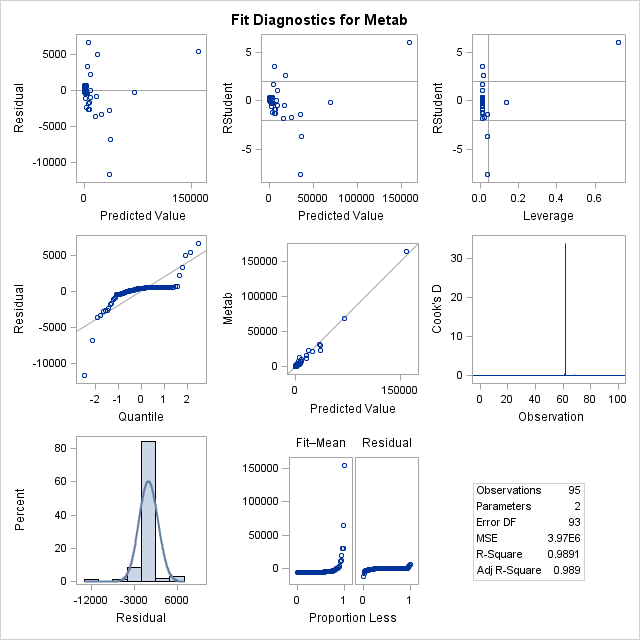
\includegraphics[scale=.8]{SASout/sasassraw.png}
	\end{center}
\caption*{The first two plots,the residuals vs predicted values and the studentized residuals vs predicted values, show us that a lot of our residuals are extreme values. The Q-Q plot and histogram tells us are residuals are not normally distributed at all, which is pretty evident.}
\end{figure}
\begin{figure}[H]
	\caption{Fit Plot}
	\label{fig:SASfitRaw}
	\begin{center}
		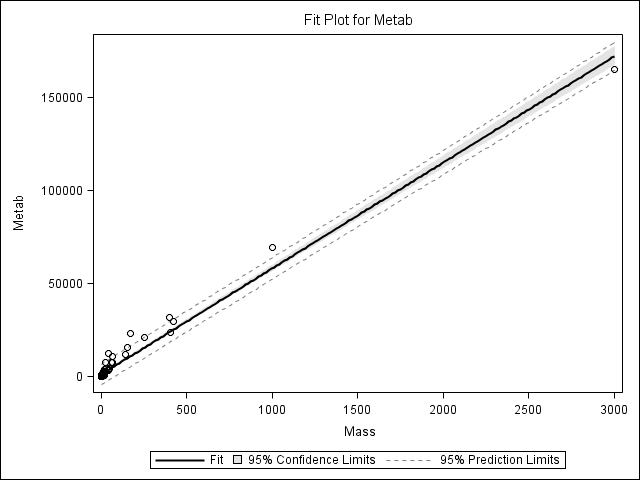
\includegraphics[scale=0.6]{SASout/sasassraw2.png}
	\end{center}
\caption*{This scatterplot of our data with a linear fit as well as confidence and prediction intervals tells us our data is not very linear, as it is not a random cloud about the fit line.}
\end{figure}
\begin{figure}[H]
	\caption{Residual vs Independent Variable Plot}
	\label{fig:SASvarraw}
	\begin{center}
		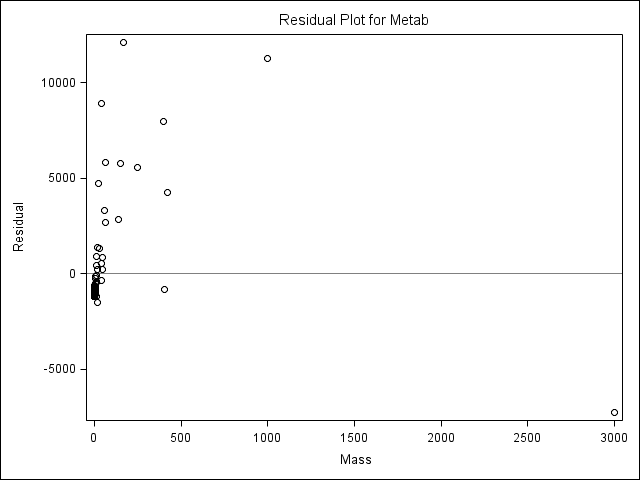
\includegraphics[scale=0.6]{SASout/sasassraw1.png}
	\end{center}
\caption*{It is increasingly evident that our data is not linear, as the residuals do not follow a linear pattern at all, not clouding about the x axis. It is also evident, from the distance of the residuals to the x axis, that they do not have a constant variance/spread at all, which is not a good sign for the no-log model}
\end{figure}
It is clear from Figures \ref{fig:SASdiagraw}, \ref{fig:SASvarraw}, and \ref{fig:SASfitRaw} that the linear (no-log) model does not work. It is not linear, does not have constant variance/equal spread, and it is in no way normal. We will try a log-log transformation on the data to see if we can improve things! To do this we will use the following SAS code:
\begin{Code}[H]
	\caption{Log-Log Transformation in SAS}
	\label{cd:loglog}
\begin{knitrout}
\definecolor{shadecolor}{rgb}{0.969, 0.969, 0.969}\color{fgcolor}\begin{kframe}
\begin{alltt}
data logmetabolism;
set powermetabolism;
logMass=log(powerMass);
logMetab=log(Metab);
run;
proc glm data=logmetabolism plots=all;
model logMetab=logMass /CLPARM;
run;
\end{alltt}
\end{kframe}
\end{knitrout}
\end{Code}
To test our assumptions, we will examine the following figures, produced by Code \ref{cd:loglog}:

\begin{figure}[H]
	\caption{Diagnostic Plots of the Log-Log Transformed Data}
	\label{fig:SASdiagrlog}
	\begin{center}
		\includegraphics[scale=.8]{SASout/saslog.png}
	\end{center}
	\caption*{The first two plots,the residuals vs predicted values and the studentized residuals vs predicted values, show us that we do not have a lot of extreme values. The Q-Q plot and histogram tells us are residuals are pretty normally distributed.}
\end{figure}
\begin{figure}[H]
	\caption{Fit Plot of the Log-Log Transformed Data}
	\label{fig:SASfitlog}
	\begin{center}
		\includegraphics[scale=0.6]{SASout/saslog2.png}
	\end{center}
	\caption*{This scatterplot of our data with a linear fit as well as confidence and prediction intervals tells us our data is pretty linear, a random cloud about the line within reasonable intervals.}
\end{figure}
\begin{figure}[H]
	\caption{Residual vs Independent Variable Plot of the Log-Log Transformed Data}
	\label{fig:SASvarlog}
	\begin{center}
		\includegraphics[scale=0.6]{SASout/saslog1.png}
	\end{center}
	\caption*{It is increasingly evident that our data is linear, as the residuals cloud about the x axis. It is also evident, from the distance of upper residuals to the lower ones, that they have an equal spread/constant variance.}
\end{figure}
It is clear from Figures \ref{fig:SASdiagrlog}, \ref{fig:SASvarlog}, and \ref{fig:SASfitlog} that the log-log model meets the assumptions of constant variance, normality, and linearity. We will assume independence.
\subsection{Assessment of the Model}
To assess our model, we will look at the p values and t statistics of the regression parameters. Those were produced in Code \ref{cd:loglog}, and are displayed in the following table:
% latex table generated in R 3.5.1 by xtable 1.8-3 package
% Sun Nov 11 22:23:01 2018
\begin{table}[H]
\centering
\caption{p-Values and T-statistics of Regression Parameters} 
\label{tab:ptsas}
\begin{tabular}{rlllllll}
  \toprule
 & Parameter & Estimate & Standard Error & t-Statistic & p-Value & Lower CI & Upper CI \\ 
  \midrule
1 & Intercept & 5.638330664 & 0.04709325 & 119.73 & $<$.0001 & 5.544812798 & 5.731848530 \\ 
  2 & logMass & 0.984991519 & 0.01949275 & 50.53 & $<$.0001 & 0.946282773 & 1.023700265 \\ 
   \bottomrule
\end{tabular}
\end{table}


From table \ref{tab:ptsas}, it is clear to see that both our intercept and slope are statistically significant!
\subsection{Regression Equation}
The regression equation is $$ \mathrm{ln}\left(\widehat{\mathrm{metabolism}}\right)=5.638330664+0.984991519\mathrm{ln}\left(\widehat{\mathrm{mass}}^{\frac{3}{4}}\right)$$
By unlogging (or raising e to everything), we can untransform the data. That is:
 $$e^{\mathrm{ln}\left(\widehat{\mathrm{metabolism}}\right)}=e^{5.638330664+0.984991519\mathrm{ln}\left(\widehat{\mathrm{mass}}^{\frac{3}{4}}\right)}=e^{5.638330664}e^{\left[\mathrm{ln}\left(\widehat{\mathrm{mass}}^{\frac{3}{4}}\right)\right]^{0.984991519}}$$
Or
$$\widehat{\mathrm{metabolism}}=e^{5.638330664}\left(\widehat{\mathrm{mass}}^{\frac{3}{4}}\right)^{0.984991519}$$
I am still not sure why we are testing it this way... Why do we not just use the normal mass and see if the exponent is .75 or not? 
\subsection{Interpretation}
The model states that the natural log of metabolism is equal to $5.638330664$ plus $0.984991519$ times the natural log of mass to three quarters. That says that if the natural log of mass to three over four were to increase by 1, the natural log of metabolism would increase by almost 1. If we unlog, we can say that a 1\% increase in mass to the three quarters leads to a .985\% increase in metabolism. A 95\% confidence interval for this is $\left[0.946282773,1.023700265\right]$, meaning that a 1\% increase in mass to the three quarters leads to a percent increase in the \emph{median} of metabolism between those two values. The problem did not ask for a confidence interval on the intercept but you can see it in Table \ref{tab:ptsas}. Because one is contained in the confidence interval, we can say that mass to the three quarters is a good estimate of the metabolism.
\subsection{Proportions}
% latex table generated in R 3.5.1 by xtable 1.8-3 package
% Sun Nov 11 22:23:01 2018
\begin{table}[H]
\centering
\caption{Proportion explained by the model} 
\label{tab:prop}
\begin{tabular}{rllll}
  \toprule
 & R-Square & Coeff Var & Root MSE & logMetab Mean \\ 
  \midrule
1 & 0.964858 & 7.819557 & 0.457235 & 5.847322 \\ 
   \bottomrule
\end{tabular}
\end{table}

$R^2$ is 0.965, which means 96.5\% of the variation is explained by the model. A good fit! Well done mr. Kleiber!
\section{Autism Study}
\subsection{Assumption Checking}
To check the assumptions of the \emph{raw} data, the following R Code was used:
\begin{Code}[H]
	\caption{Plotting the Raw Data in R}
\begin{knitrout}
\definecolor{shadecolor}{rgb}{0.969, 0.969, 0.969}\color{fgcolor}\begin{kframe}
\begin{alltt}
\hlstd{data}\hlkwb{<-}\hlkwd{read.csv}\hlstd{(}\hlstr{"Data/Autism.csv"}\hlstd{)}
\hlstd{data}\hlkwb{<-}\hlstd{data}\hlopt\hlkwd{mutate}\hlstd{(}\hlkwc{logPrevalence}\hlstd{=}\hlkwd{log}\hlstd{(Prevalence))}
\hlstd{model1} \hlkwb{<-}\hlkwd{lm}\hlstd{(Prevalence}\hlopt{~}\hlstd{Year,}\hlkwc{data}\hlstd{=data)}
\hlstd{pint}\hlkwb{<-}\hlkwd{predict}\hlstd{(model1,}\hlkwc{interval}\hlstd{=}\hlstr{"prediction"}\hlstd{,}\hlkwc{level}\hlstd{=}\hlnum{.95}\hlstd{)}
\hlstd{new_df}\hlkwb{<-}\hlkwd{cbind}\hlstd{(data,pint)}
\hlstd{g}\hlkwb{<-}\hlkwd{ggplot}\hlstd{(new_df,} \hlkwd{aes}\hlstd{(}\hlkwc{x}\hlstd{=Year,} \hlkwc{y}\hlstd{=Prevalence))}\hlopt{+}\hlkwd{geom_point}\hlstd{()} \hlopt{+}
\hlkwd{geom_line}\hlstd{(}\hlkwd{aes}\hlstd{(}\hlkwc{y}\hlstd{=lwr),} \hlkwc{color} \hlstd{=} \hlstr{"red"}\hlstd{,} \hlkwc{linetype} \hlstd{=} \hlstr{"dashed"}\hlstd{)}\hlopt{+}
\hlkwd{geom_line}\hlstd{(}\hlkwd{aes}\hlstd{(}\hlkwc{y}\hlstd{=upr),} \hlkwc{color} \hlstd{=} \hlstr{"red"}\hlstd{,} \hlkwc{linetype} \hlstd{=} \hlstr{"dashed"}\hlstd{)}\hlopt{+}
\hlkwd{geom_smooth}\hlstd{(}\hlkwc{method}\hlstd{=lm,} \hlkwc{se}\hlstd{=}\hlnum{TRUE}\hlstd{,}\hlkwc{level}\hlstd{=}\hlnum{0.95}\hlstd{)}\hlopt{+}
\hlkwd{theme_classic}\hlstd{()}
\hlstd{resp}\hlkwb{<-}\hlkwd{ggplot}\hlstd{(model1,} \hlkwd{aes}\hlstd{(.fitted, .resid))}\hlopt{+}
\hlkwd{geom_point}\hlstd{(}\hlkwd{aes}\hlstd{(}\hlkwc{color} \hlstd{= .resid))} \hlopt{+}
\hlkwd{scale_color_gradient2}\hlstd{(}\hlkwc{low} \hlstd{=} \hlstr{"blue"}\hlstd{,}
\hlkwc{mid} \hlstd{=} \hlstr{"gray"}\hlstd{,}
\hlkwc{high} \hlstd{=} \hlstr{"red"}\hlstd{)} \hlopt{+}
\hlkwd{guides}\hlstd{(}\hlkwc{color} \hlstd{=} \hlnum{FALSE}\hlstd{)}
\hlstd{resp}\hlkwb{<-}\hlstd{resp}\hlopt{+}
\hlkwd{stat_smooth}\hlstd{(}\hlkwc{method}\hlstd{=}\hlstr{"lm"}\hlstd{,}\hlkwc{se}\hlstd{=F)}\hlopt{+}
\hlkwd{geom_hline}\hlstd{(}\hlkwc{yintercept}\hlstd{=}\hlnum{0}\hlstd{,}
\hlkwc{col}\hlstd{=}\hlstr{"red"}\hlstd{,}
\hlkwc{linetype}\hlstd{=}\hlstr{"dashed"}\hlstd{)}
\hlstd{resp}\hlkwb{<-}\hlstd{resp}\hlopt{+}
\hlkwd{xlab}\hlstd{(}\hlstr{"Fitted values"}\hlstd{)}\hlopt{+}
\hlkwd{ylab}\hlstd{(}\hlstr{"Residuals"}\hlstd{)}
\hlstd{resp}\hlkwb{<-}\hlstd{resp}\hlopt{+}\hlkwd{theme_classic}\hlstd{()}\hlopt{+}\hlkwd{geom_segment}\hlstd{(}\hlkwd{aes}\hlstd{(}\hlkwc{y}\hlstd{=}\hlnum{0}\hlstd{,}\hlkwc{x}\hlstd{=.fitted,}\hlkwc{xend}\hlstd{=.fitted,} \hlkwc{yend}\hlstd{=.resid,}
\hlkwc{alpha} \hlstd{=} \hlnum{2}\hlopt{*}\hlkwd{abs}\hlstd{(.resid)))}\hlopt{+}\hlkwd{guides}\hlstd{(}\hlkwc{alpha}\hlstd{=}\hlnum{FALSE}\hlstd{)}
\hlstd{resx}\hlkwb{<-}\hlkwd{ggplot}\hlstd{(model1,} \hlkwd{aes}\hlstd{(Year, .resid))}\hlopt{+}
\hlkwd{geom_point}\hlstd{(}\hlkwd{aes}\hlstd{(}\hlkwc{color} \hlstd{= .resid))} \hlopt{+}
\hlkwd{scale_color_gradient2}\hlstd{(}\hlkwc{low} \hlstd{=} \hlstr{"blue"}\hlstd{,}
\hlkwc{mid} \hlstd{=} \hlstr{"gray"}\hlstd{,}
\hlkwc{high} \hlstd{=} \hlstr{"red"}\hlstd{)} \hlopt{+}
\hlkwd{guides}\hlstd{(}\hlkwc{color} \hlstd{=} \hlnum{FALSE}\hlstd{)}
\hlstd{resx}\hlkwb{<-}\hlstd{resx}\hlopt{+}
\hlkwd{stat_smooth}\hlstd{(}\hlkwc{method}\hlstd{=}\hlstr{"lm"}\hlstd{,}\hlkwc{se}\hlstd{=F)}\hlopt{+}
\hlkwd{geom_hline}\hlstd{(}\hlkwc{yintercept}\hlstd{=}\hlnum{0}\hlstd{,}
\hlkwc{col}\hlstd{=}\hlstr{"red"}\hlstd{,}
\hlkwc{linetype}\hlstd{=}\hlstr{"dashed"}\hlstd{)}
\hlstd{resx}\hlkwb{<-}\hlstd{resx}\hlopt{+}
\hlkwd{xlab}\hlstd{(}\hlstr{"Year"}\hlstd{)}\hlopt{+}
\hlkwd{ylab}\hlstd{(}\hlstr{"Residuals"}\hlstd{)}
\hlstd{resx}\hlkwb{<-}\hlstd{resx}\hlopt{+}\hlkwd{theme_classic}\hlstd{()}\hlopt{+}\hlkwd{geom_segment}\hlstd{(}\hlkwd{aes}\hlstd{(}\hlkwc{y}\hlstd{=}\hlnum{0}\hlstd{,}\hlkwc{x}\hlstd{=Year,}\hlkwc{xend}\hlstd{=Year,} \hlkwc{yend}\hlstd{=.resid,}
\hlkwc{alpha} \hlstd{=} \hlnum{2}\hlopt{*}\hlkwd{abs}\hlstd{(.resid)))}\hlopt{+}\hlkwd{guides}\hlstd{(}\hlkwc{alpha}\hlstd{=}\hlnum{FALSE}\hlstd{)}
\hlstd{extraVal}\hlkwb{<-}\hlkwd{fortify}\hlstd{(model1)}
\hlstd{ghist}\hlkwb{<-}\hlkwd{ggplot}\hlstd{(model1,}\hlkwd{aes}\hlstd{(}\hlkwc{x}\hlstd{=.resid))}\hlopt{+}
\hlkwd{geom_histogram}\hlstd{(}\hlkwc{bins}\hlstd{=}\hlnum{4}\hlstd{,}
\hlkwc{fill}\hlstd{=}\hlstr{'gray22'}\hlstd{,}
\hlkwc{color}\hlstd{=}\hlstr{'ghostwhite'}\hlstd{)}\hlopt{+}
\hlkwd{theme_classic}\hlstd{()}
\hlstd{ghist}\hlkwb{<-}\hlstd{ghist}\hlopt{+}\hlkwd{stat_function}\hlstd{(}\hlkwc{fun}\hlstd{=dnorm,}
\hlkwc{color}\hlstd{=}\hlstr{"forestgreen"}\hlstd{,}\hlkwc{args}\hlstd{=}\hlkwd{list}\hlstd{(}\hlkwc{mean}\hlstd{=}\hlkwd{mean}\hlstd{(extraVal}\hlopt{$}\hlstd{.resid),}
\hlkwc{sd}\hlstd{=}\hlkwd{sd}\hlstd{(extraVal}\hlopt{$}\hlstd{.resid)),}\hlkwc{size}\hlstd{=}\hlnum{1}\hlstd{)}
\end{alltt}
\end{kframe}
\end{knitrout}
\end{Code}
This results in the following figures:
\begin{figure}[H]
	\caption{Plot of the Raw Fit}
	\begin{center}
\begin{knitrout}
\definecolor{shadecolor}{rgb}{0.969, 0.969, 0.969}\color{fgcolor}
\includegraphics[width=\maxwidth]{figure/fit_plotraw-1} 

\end{knitrout}
\par\end{center}
\end{figure}
\begin{figure}[H]
	\caption{Plot of the Raw Residuals vs Fitted Values}
	\begin{center}
\begin{knitrout}
\definecolor{shadecolor}{rgb}{0.969, 0.969, 0.969}\color{fgcolor}
\includegraphics[width=\maxwidth]{figure/resid_plotraw-1} 

\end{knitrout}
\par\end{center}
\end{figure}

\begin{figure}[H]
	\begin{center}
	\caption{Plot of the Raw Residuals vs Year}
\begin{knitrout}
\definecolor{shadecolor}{rgb}{0.969, 0.969, 0.969}\color{fgcolor}
\includegraphics[width=\maxwidth]{figure/residx_plotraw-1} 

\end{knitrout}
	\par\end{center}
\end{figure}
\begin{figure}[H]
	\caption{Histogram of the Raw Residuals}
	\begin{center}
\begin{knitrout}
\definecolor{shadecolor}{rgb}{0.969, 0.969, 0.969}\color{fgcolor}
\includegraphics[width=\maxwidth]{figure/resid_histraw-1} 

\end{knitrout}
	\par\end{center}
\end{figure}
As we can see, this data needs to be transformed! Lets log transform the Y axis! We do this with the following Code:
\begin{Code}[H]
	\caption{Plotting the Log-Linear Data in R}
\begin{knitrout}
\definecolor{shadecolor}{rgb}{0.969, 0.969, 0.969}\color{fgcolor}\begin{kframe}
\begin{alltt}
\hlstd{model2} \hlkwb{<-}\hlkwd{lm}\hlstd{(logPrevalence}\hlopt{~}\hlstd{Year,}\hlkwc{data}\hlstd{=data)}
\hlstd{pint2}\hlkwb{<-}\hlkwd{predict}\hlstd{(model2,}\hlkwc{interval}\hlstd{=}\hlstr{"prediction"}\hlstd{,}\hlkwc{level}\hlstd{=}\hlnum{.95}\hlstd{)}
\hlstd{new_df}\hlkwb{<-}\hlkwd{cbind}\hlstd{(data,pint2)}
\hlstd{g2}\hlkwb{<-}\hlkwd{ggplot}\hlstd{(new_df,} \hlkwd{aes}\hlstd{(}\hlkwc{x}\hlstd{=Year,} \hlkwc{y}\hlstd{=logPrevalence))}\hlopt{+}\hlkwd{geom_point}\hlstd{()} \hlopt{+}
\hlkwd{geom_line}\hlstd{(}\hlkwd{aes}\hlstd{(}\hlkwc{y}\hlstd{=lwr),} \hlkwc{color} \hlstd{=} \hlstr{"red"}\hlstd{,} \hlkwc{linetype} \hlstd{=} \hlstr{"dashed"}\hlstd{)}\hlopt{+}
\hlkwd{geom_line}\hlstd{(}\hlkwd{aes}\hlstd{(}\hlkwc{y}\hlstd{=upr),} \hlkwc{color} \hlstd{=} \hlstr{"red"}\hlstd{,} \hlkwc{linetype} \hlstd{=} \hlstr{"dashed"}\hlstd{)}\hlopt{+}
\hlkwd{geom_smooth}\hlstd{(}\hlkwc{method}\hlstd{=lm,} \hlkwc{se}\hlstd{=}\hlnum{TRUE}\hlstd{,}\hlkwc{level}\hlstd{=}\hlnum{0.95}\hlstd{)}\hlopt{+}
\hlkwd{theme_classic}\hlstd{()}
\hlstd{resp2}\hlkwb{<-}\hlkwd{ggplot}\hlstd{(model2,} \hlkwd{aes}\hlstd{(.fitted, .resid))}\hlopt{+}
\hlkwd{geom_point}\hlstd{(}\hlkwd{aes}\hlstd{(}\hlkwc{color} \hlstd{= .resid))} \hlopt{+}
\hlkwd{scale_color_gradient2}\hlstd{(}\hlkwc{low} \hlstd{=} \hlstr{"blue"}\hlstd{,}
\hlkwc{mid} \hlstd{=} \hlstr{"gray"}\hlstd{,}
\hlkwc{high} \hlstd{=} \hlstr{"red"}\hlstd{)} \hlopt{+}
\hlkwd{guides}\hlstd{(}\hlkwc{color} \hlstd{=} \hlnum{FALSE}\hlstd{)}
\hlstd{resp2}\hlkwb{<-}\hlstd{resp2}\hlopt{+}
\hlkwd{stat_smooth}\hlstd{(}\hlkwc{method}\hlstd{=}\hlstr{"lm"}\hlstd{,}\hlkwc{se}\hlstd{=F)}\hlopt{+}
\hlkwd{geom_hline}\hlstd{(}\hlkwc{yintercept}\hlstd{=}\hlnum{0}\hlstd{,}
\hlkwc{col}\hlstd{=}\hlstr{"red"}\hlstd{,}
\hlkwc{linetype}\hlstd{=}\hlstr{"dashed"}\hlstd{)}
\hlstd{resp2}\hlkwb{<-}\hlstd{resp2}\hlopt{+}
\hlkwd{xlab}\hlstd{(}\hlstr{"Fitted values"}\hlstd{)}\hlopt{+}
\hlkwd{ylab}\hlstd{(}\hlstr{"Residuals"}\hlstd{)}
\hlstd{resp2}\hlkwb{<-}\hlstd{resp2}\hlopt{+}\hlkwd{theme_classic}\hlstd{()}\hlopt{+}\hlkwd{geom_segment}\hlstd{(}\hlkwd{aes}\hlstd{(}\hlkwc{y}\hlstd{=}\hlnum{0}\hlstd{,}\hlkwc{x}\hlstd{=.fitted,}\hlkwc{xend}\hlstd{=.fitted,} \hlkwc{yend}\hlstd{=.resid,}
\hlkwc{alpha} \hlstd{=} \hlnum{2}\hlopt{*}\hlkwd{abs}\hlstd{(.resid)))}\hlopt{+}\hlkwd{guides}\hlstd{(}\hlkwc{alpha}\hlstd{=}\hlnum{FALSE}\hlstd{)}
\hlstd{resx2}\hlkwb{<-}\hlkwd{ggplot}\hlstd{(model2,} \hlkwd{aes}\hlstd{(Year, .resid))}\hlopt{+}
\hlkwd{geom_point}\hlstd{(}\hlkwd{aes}\hlstd{(}\hlkwc{color} \hlstd{= .resid))} \hlopt{+}
\hlkwd{scale_color_gradient2}\hlstd{(}\hlkwc{low} \hlstd{=} \hlstr{"blue"}\hlstd{,}
\hlkwc{mid} \hlstd{=} \hlstr{"gray"}\hlstd{,}
\hlkwc{high} \hlstd{=} \hlstr{"red"}\hlstd{)} \hlopt{+}
\hlkwd{guides}\hlstd{(}\hlkwc{color} \hlstd{=} \hlnum{FALSE}\hlstd{)}
\hlstd{resx2}\hlkwb{<-}\hlstd{resx2}\hlopt{+}
\hlkwd{stat_smooth}\hlstd{(}\hlkwc{method}\hlstd{=}\hlstr{"lm"}\hlstd{,}\hlkwc{se}\hlstd{=F)}\hlopt{+}
\hlkwd{geom_hline}\hlstd{(}\hlkwc{yintercept}\hlstd{=}\hlnum{0}\hlstd{,}
\hlkwc{col}\hlstd{=}\hlstr{"red"}\hlstd{,}
\hlkwc{linetype}\hlstd{=}\hlstr{"dashed"}\hlstd{)}
\hlstd{resx2}\hlkwb{<-}\hlstd{resx2}\hlopt{+}
\hlkwd{xlab}\hlstd{(}\hlstr{"Year"}\hlstd{)}\hlopt{+}
\hlkwd{ylab}\hlstd{(}\hlstr{"Residuals"}\hlstd{)}
\hlstd{resx2}\hlkwb{<-}\hlstd{resx2}\hlopt{+}\hlkwd{theme_classic}\hlstd{()}\hlopt{+}\hlkwd{geom_segment}\hlstd{(}\hlkwd{aes}\hlstd{(}\hlkwc{y}\hlstd{=}\hlnum{0}\hlstd{,}\hlkwc{x}\hlstd{=Year,}\hlkwc{xend}\hlstd{=Year,} \hlkwc{yend}\hlstd{=.resid,}
\hlkwc{alpha} \hlstd{=} \hlnum{2}\hlopt{*}\hlkwd{abs}\hlstd{(.resid)))}\hlopt{+}\hlkwd{guides}\hlstd{(}\hlkwc{alpha}\hlstd{=}\hlnum{FALSE}\hlstd{)}
\hlstd{extraVal2}\hlkwb{<-}\hlkwd{fortify}\hlstd{(model2)}
\hlstd{ghist2}\hlkwb{<-}\hlkwd{ggplot}\hlstd{(model2,}\hlkwd{aes}\hlstd{(}\hlkwc{x}\hlstd{=.resid))}\hlopt{+}
\hlkwd{geom_histogram}\hlstd{(}\hlkwc{bins}\hlstd{=}\hlnum{4}\hlstd{,}
\hlkwc{fill}\hlstd{=}\hlstr{'gray22'}\hlstd{,}
\hlkwc{color}\hlstd{=}\hlstr{'ghostwhite'}\hlstd{)}\hlopt{+}
\hlkwd{theme_classic}\hlstd{()}
\hlstd{ghist2}\hlkwb{<-}\hlstd{ghist2}\hlopt{+}\hlkwd{stat_function}\hlstd{(}\hlkwc{fun}\hlstd{=dnorm,}
\hlkwc{color}\hlstd{=}\hlstr{"forestgreen"}\hlstd{,}\hlkwc{args}\hlstd{=}\hlkwd{list}\hlstd{(}\hlkwc{mean}\hlstd{=}\hlkwd{mean}\hlstd{(extraVal2}\hlopt{$}\hlstd{.resid),}
\hlkwc{sd}\hlstd{=}\hlkwd{sd}\hlstd{(extraVal2}\hlopt{$}\hlstd{.resid)),}\hlkwc{size}\hlstd{=}\hlnum{1}\hlstd{)}
\end{alltt}
\end{kframe}
\end{knitrout}
	\end{Code}
	\begin{figure}[H]
		\caption{Plot of the Logged Fit}
		\begin{center}
\begin{knitrout}
\definecolor{shadecolor}{rgb}{0.969, 0.969, 0.969}\color{fgcolor}
\includegraphics[width=\maxwidth]{figure/fit_plotlog-1} 

\end{knitrout}
			\par\end{center}
	\end{figure}
	\begin{figure}[H]
		\caption{Plot of the Logged Residuals vs Fitted Values}
		\begin{center}
\begin{knitrout}
\definecolor{shadecolor}{rgb}{0.969, 0.969, 0.969}\color{fgcolor}
\includegraphics[width=\maxwidth]{figure/resid_plotlog-1} 

\end{knitrout}
			\par\end{center}
	\end{figure}
	
	\begin{figure}[H]
		\begin{center}
			\caption{Plot of the Logged Residuals vs Year}
\begin{knitrout}
\definecolor{shadecolor}{rgb}{0.969, 0.969, 0.969}\color{fgcolor}
\includegraphics[width=\maxwidth]{figure/residx_plotlog-1} 

\end{knitrout}
			\par\end{center}
	\end{figure}
	\begin{figure}[H]
		\caption{Histogram of the Logged Residuals}
		\begin{center}
\begin{knitrout}
\definecolor{shadecolor}{rgb}{0.969, 0.969, 0.969}\color{fgcolor}
\includegraphics[width=\maxwidth]{figure/resid_histlog-1} 

\end{knitrout}
			\par\end{center}
	\end{figure}
This is a way better fit!
\subsection{Model Assessment}
Lets look at the model parameters!
% latex table generated in R 3.5.1 by xtable 1.8-3 package
% Sun Nov 11 23:43:33 2018
\begin{table}[H]
\centering
\caption{Hypothesis Test on Regression Parameters} 
\label{tb:betas}
\begin{tabular}{rlrrrrrr}
  \toprule
 & term & estimate & std.error & statistic & p.value & conf.low & conf.high \\ 
  \midrule
1 & (Intercept) & -407.98 & 4.95 & -82.38 & 0.00 & -423.74 & -392.21 \\ 
  2 & Year & 0.21 & 0.00 & 82.79 & 0.00 & 0.20 & 0.21 \\ 
   \bottomrule
\end{tabular}
\end{table}

\subsection{Regression Equation}
The regression equation is:
$$\mathrm{ln}\left(\widehat{\mathrm{Prevalence}}\right)=-408+.21\left(\widehat{\mathrm{Year}}\right)$$
\subsection{Interpretation}
A one unit increase in Year is associated with a multiplicative change of $e^.21$ in the median of Prevalence. A confidence interval for this is shown in Table 3, it is very narrow.
\subsection{R squared}
\begin{knitrout}
\definecolor{shadecolor}{rgb}{0.969, 0.969, 0.969}\color{fgcolor}\begin{kframe}
\begin{alltt}
\hlstd{rsquare}\hlkwb{<-}\hlkwd{summary}\hlstd{(model2)}\hlopt{$}\hlstd{r.squared}
\end{alltt}
\end{kframe}
\end{knitrout}
$R^2=0.9995625$
\end{document}
